\section{Derivation of the analytic posterior for toy example}
\label{sec:analytical_posterior}

In this appendix we derive and compute the conditional distribution \(\Fcond\) for the toy example of \autoref{sec:toy_example}.
We denote by \(f_i(\cdot)\) and \(F_i(\cdot)\) the prior probability distribution function and cumulative distribution function of \(X_i\), i.e. the normal PDF and CDF with means and variances given by \autoref{eq:toyspec}.
Let \(\pij\) be the probability that \(X_i\) is the minimum of \(X\) and \(X_j\) is its maximum.
We also define \(\pisum = \sum_{j=1}^{100} \pij\), the probability that \(X_i\) is the minimum,
and \(\psumj = \sum_{i=1}^{100} \pij\), the probability that \(X_j\) is the maximum.
The cumulative distribution function of \(X_i\) is then given by:
\begin{equation}
\Pr\del{X_i \leq x \mid \Xmax, \Xmin} =
    \begin{cases}
        0 &\text{if } x < \Xmin \,, \\
        1 &\text{if } x \geq \Xmax \,, \\
        \pxx{i}{\bullet} 
            + \del{1 \!-\! \pxx{i}{\bullet} \!-\! \pxx{\bullet}{i}}
            \sbr{\frac{F_i(x) - F_i(\Xmin) }
                 {F_i(\Xmax) - F_i(\Xmin) }
                } 
            &\text{otherwise.}\\
    \end{cases}
\end{equation}
Meanwhile, \(\pij\) is proportional to:
\begin{equation}
    f_i(\Xmin)
    f_j(\Xmax)
    \prod_{k \neq i,j}^{100}
    \del{F_k(\Xmax) - F_k(\Xmin)} \,,
\end{equation}
which we compute for all \(i,j\) and normalize
to obtain the \(100 \times 100\) matrix \(\Pr\) of probabilities of each pair of element occupying the extremes.
We sum over its rows and columns to obtain \(\psumj\) and \(\pisum\).
While this algorithm has cubic complexity in the dimensionality \(p\) of \(X\),
for \(p=100\), it only take seconds to compute the entries of \(\Pr\) and evaluate \(\Pr\del{X_i \leq x \mid \Xmax, \Xmin}\) over a range of \(x\).
\autoref{fig:toy_quantiles}(b) shows the analytical quantiles of \(\Fcond\) marginally for each \(X_i\).

\section{Modeling the diurnal cycle with Gaussian processes}
\label{appendix:diurnal_kernel}

Reviewers of earlier versions of this paper have raised concerns about our use of a periodic kernel,
instead of a periodic mean function in \autoref{eq:kdiurn} and \autoref{eq:sumprod_kernel}.
It is indeed commonplace in geostatistics to specify a mean functions that is the sum of harmonics
with a period of 24 hours (diurnal cycle) or 365 days (seasonal cycle) and integer fractions thereof:
\begin{equation}
    m(t) = \sum_{w=1}^W \sbr{a_w \cos(2\pi t w / 24) + b_w \sin(2\pi t w / 24)}
    \label{eq:mperiodic}
\end{equation}
with $W$ typically chosen to be between 1 and 5, and coefficients fitted by maximizing the marginal likelihood.
For example, this is the approach taken (with $W=1$) to model the seasonal component in a closely related application by \citet{kleiber2013daily}.
Since the mean function is frequently interpreted as capturing long-term trends (climate component), while the Gaussian process captures stochastic deviations from the trend (weather component), it is perceived as a natural choice to incorporate periodic components in the mean function.
However common, this narrative clashes with a Bayesian understanding of the Gaussian process.
Rather than optimizing the ($a_w,b_w$) coefficients, a Bayesian would generally prefer to equip them with priors,
and propagate their uncertainty to inferences and predictions.
A relatively uncontroversial choice would be an independent normal prior $\normal(0, \sigma^2)$ on each coefficient, 
but then it is noticed that this induces a covariance between $m(t)$ and $m(t')$ of 
$\sigma^2 \sum_{w=1}^W 
        \sbr{
            \cos(2\pi t w / 24) \cos(2\pi t' w / 24) + 
            \sin(2\pi t w / 24) \sin(2\pi t' w / 24)
            }$.
The resulting model is therefore strictly mathematically equivalent to a Gaussian process
with such a term added to the covariance kernel.
The only difference between this augmented $\GP$ 
and the mean function specification \autoref{eq:mperiodic} is that the 
uncertainty in the coefficients is now rigorously accounted for.
This reasoning holds for any linear basic function in the mean.

But rather than using this kernel derived from a finite sine and cosine basis,
we have opted to use the periodic kernel \autoref{eq:kperiodic},
which has the significant advantage of being able to fit any continuous periodic function
with only two hyperparameters (we hold the period fixed of course).
We now illustrate this advantage with a simulation from the model:
\begin{equation}
\begin{split}
    v_{24}(t) &= 5 \log\sbr{ \cos(2\pi t / 24) + 1.02} \text{, the diurnal cycle,}\\
    f(t) & \sim \GP(v_{24}(t), k(t,t')) \text{, the process,}\\
    y_i &= f(t_i) + \epsilon_i, \quad \epsilon_i \sim \normal(0, 0.1^2) \text{, the observations, }
\end{split}
\end{equation}
where time $t$ is in hours, and the $\GP$ kernel is Mat\'ern 3/2 with lengthscale 0.5 hours and variance parameter $(1.5)^2$.
We simulate 7 days of data, but withhold data from the fifth day (\autoref{fig:periodic_sim}).
We then fit the following 5 Gaussian process models:
\begin{enumerate}
    \item A constant plus periodic mean function with $W=2$ and the Mat\'ern 3/2  kernel;
    \item A constant plus periodic mean function with $W=4$ and the Mat\'ern 3/2  kernel;
    \item A constant plus periodic mean function with $W=6$ and the Mat\'ern 3/2  kernel;
    \item A constant mean function with a sum kernel of Mat\'ern 3/2 plus periodic \autoref{eq:kperiodic}.
    \item A constant plus periodic mean function with $W=2$ and a sum kernel of Mat\'ern 3/2 plus periodic.
\end{enumerate}
Each model is initialized with all mean parameters set to zero, and the Mat\'ern coefficients set to their true value,
while the periodic kernel is initialized with $\ell=1$ and variance $1$.
We then optimize the parameters and obtain predictions for the fifth day, which are shown in \autoref{fig:periodic_results}.
The resulting predictions show that the periodic kernel gives the best predictions, as the kernel was able to tightly fit the diurnal component.
The choice $W=4$ also gives good predictions, but underspecifying ($W=2$) or overspecifying ($W=6$) the mean functions leads to degraded performance.
With additional days of data, the periodic kernel will be able to fit the diurnal cycle arbitrarily well,
without necessitating additional hyperparameters.
The combination of a periodic mean function and periodic kernel does not lead to noticeably better predictions.

\begin{figure}
    \centering
    \begin{subfigure}[t]{0.32\textwidth}
    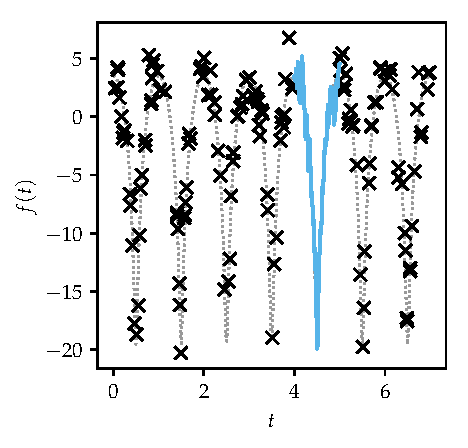
\includegraphics[width=\textwidth]{periodic/periodic_sim.pdf}
    \caption{Simulation setting}
    \label{fig:periodic_sim}
    \end{subfigure}
    \begin{subfigure}[t]{0.32\textwidth}
    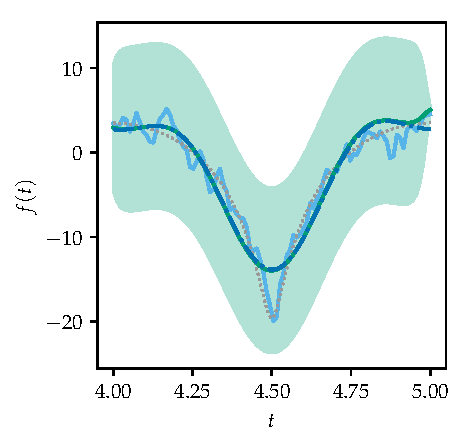
\includegraphics[width=\textwidth]{periodic/periodic_results_under.pdf}
    \caption{Periodic $m$ with $W=2$}
    \label{fig:periodic_results_under}
    \end{subfigure}
    \begin{subfigure}[t]{0.32\textwidth}
    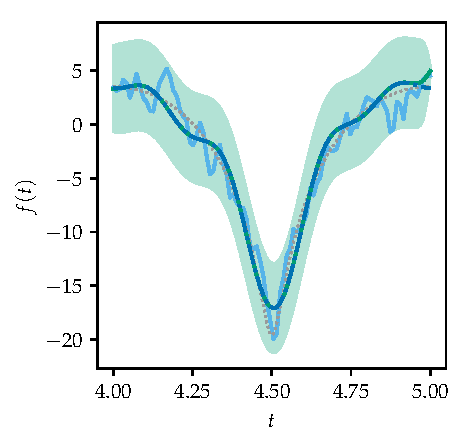
\includegraphics[width=\textwidth]{periodic/periodic_results_meanper.pdf}
    \caption{Periodic $m$ with $W=4$}
    \label{fig:periodic_results_meanper}
    \end{subfigure}
    \begin{subfigure}[t]{0.32\textwidth}
    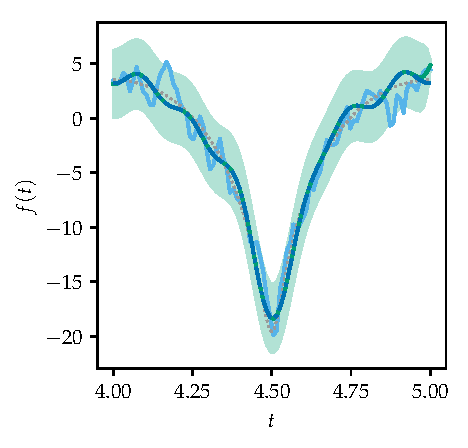
\includegraphics[width=\textwidth]{periodic/periodic_results_over.pdf}
    \caption{Periodic $m$ with $W=6$}
    \label{fig:periodic_results_over}
    \end{subfigure}
    \begin{subfigure}[t]{0.32\textwidth}
    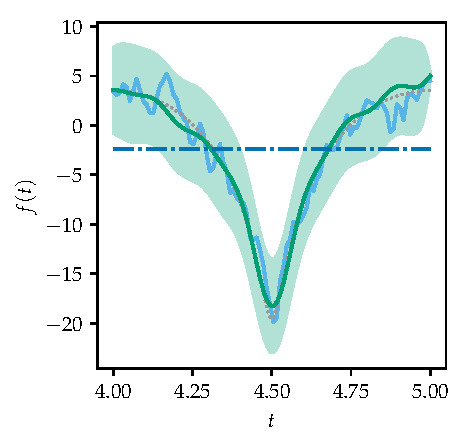
\includegraphics[width=\textwidth]{periodic/periodic_results_kper.pdf}
    \caption{Constant $m$ and periodic $k$}
    \label{fig:periodic_results_kper}
    \end{subfigure}
    \begin{subfigure}[t]{0.32\textwidth}
    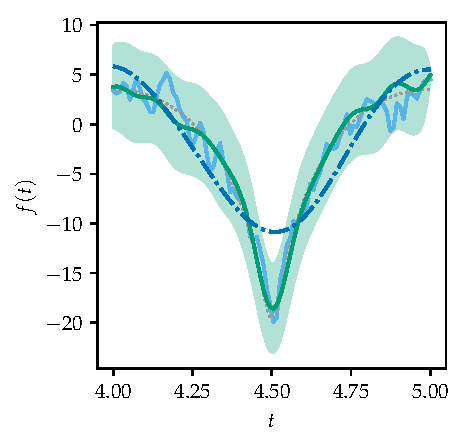
\includegraphics[width=\textwidth]{periodic/periodic_results_both.pdf}
    \caption{Periodic $m$ and periodic $k$}
    \label{fig:periodic_results_both}
    \end{subfigure}
\caption{\label{fig:periodic_results}
    Simulations comparing periodic mean functions and kernels.
    \autoref{fig:periodic_results_under} shows the observations (crosses), diurnal cycle (dotted),
    and true process in the test window (solid line).
    For each model, we show posterior mean and credible envelope (2 standard deviations),
    and the fitted mean function (dash-dotted, which often overlaps with the posterior mean).
}
\end{figure}

As an additional benefit of modeling periodic components in the kernel rather than the mean function is that drifts in the cycle (for example due to seasonal changes)
can be captured by multipling the periodic kernel with a stationary temporal kernel.
Equally, slight differences in the diurnal cycle between sites can be captured by multiplying it with a stationary spatial kernel.
